% Some LaTeX commands I define for my own nomenclature.
% If you have to, it's better to change nomenclature once here than in a 
% million places throughout your thesis!
\newcommand{\package}[1]{\textbf{#1}} % package names in bold text
\newcommand{\cmmd}[1]{\textbackslash\texttt{#1}} % command name in tt font 


%======================================================================
\chapter{Model Description}
%======================================================================

The model is composed of human population given by $N_{h}$ and
reservoir population given by $N_{r}$. We divide the human population ($N_{h}$) in $5$ categories namely, Susceptibles ($S_{h}$), Vaccinated ($V_{h}$), Exposed ($E_{h}$), Infected ($I_{h}$) and Recovered ($R_{h}$) whereas the reservoir population ($N_{r}$) is divided among Susceptibles ($S_{r}$), Infected($I_{r}$) and Recovered ($R_{r}$), such that
\[N_{h} = S_{h} + V_{h} + E_{h} + I_{h} + R_{h}\]
\[N_{r} = S_{r} + I_{r} + R_{r}\]
% FLOW DIAGRAM
\begin{figure}[h]
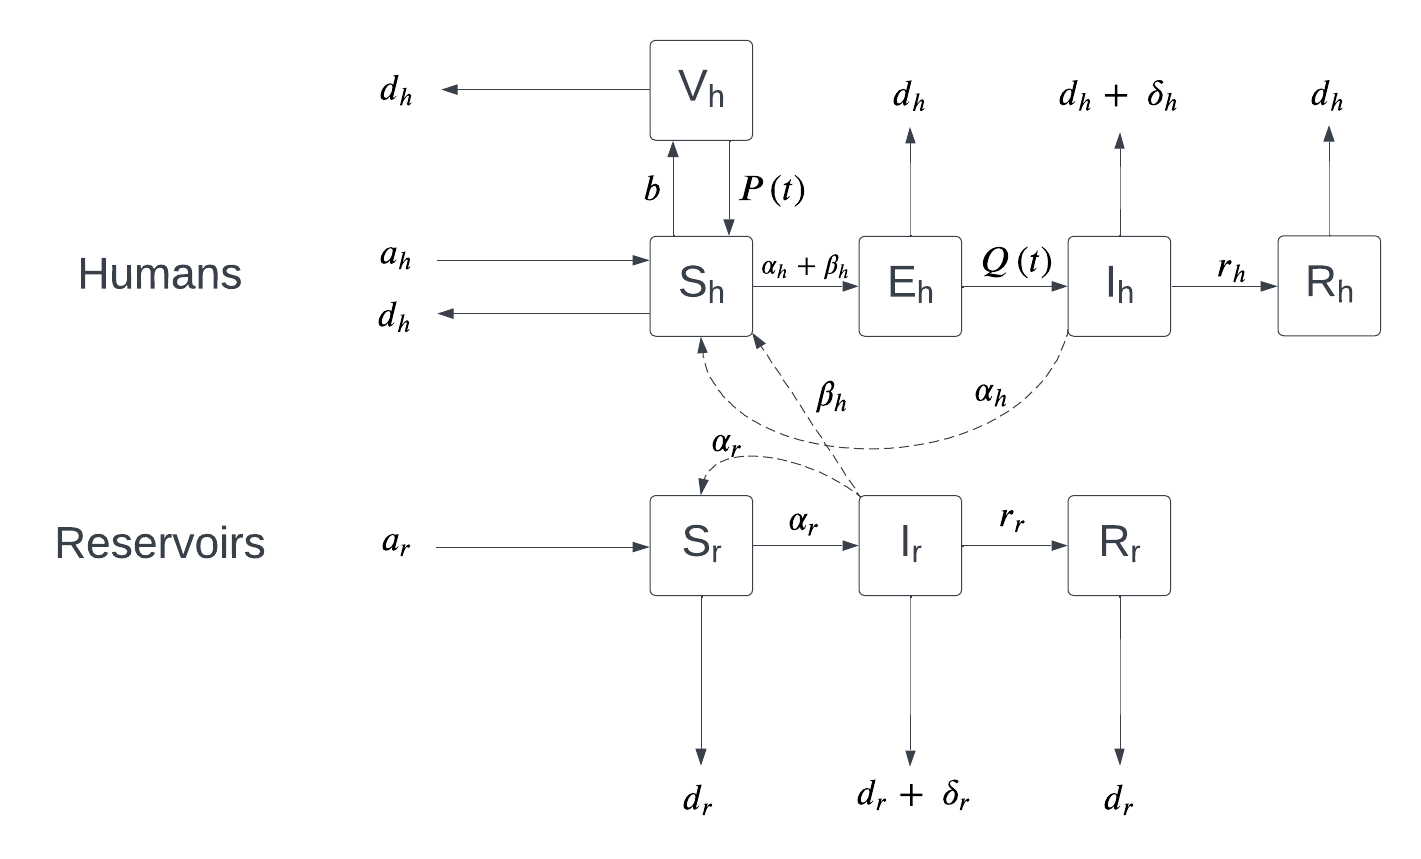
\includegraphics[width=\textwidth]{flow-diagram}
\caption{Model Flow Diagram}
\centering
\end{figure}
% PARAMETERS TABLE
\begin{figure}[h] \hspace{60pt}
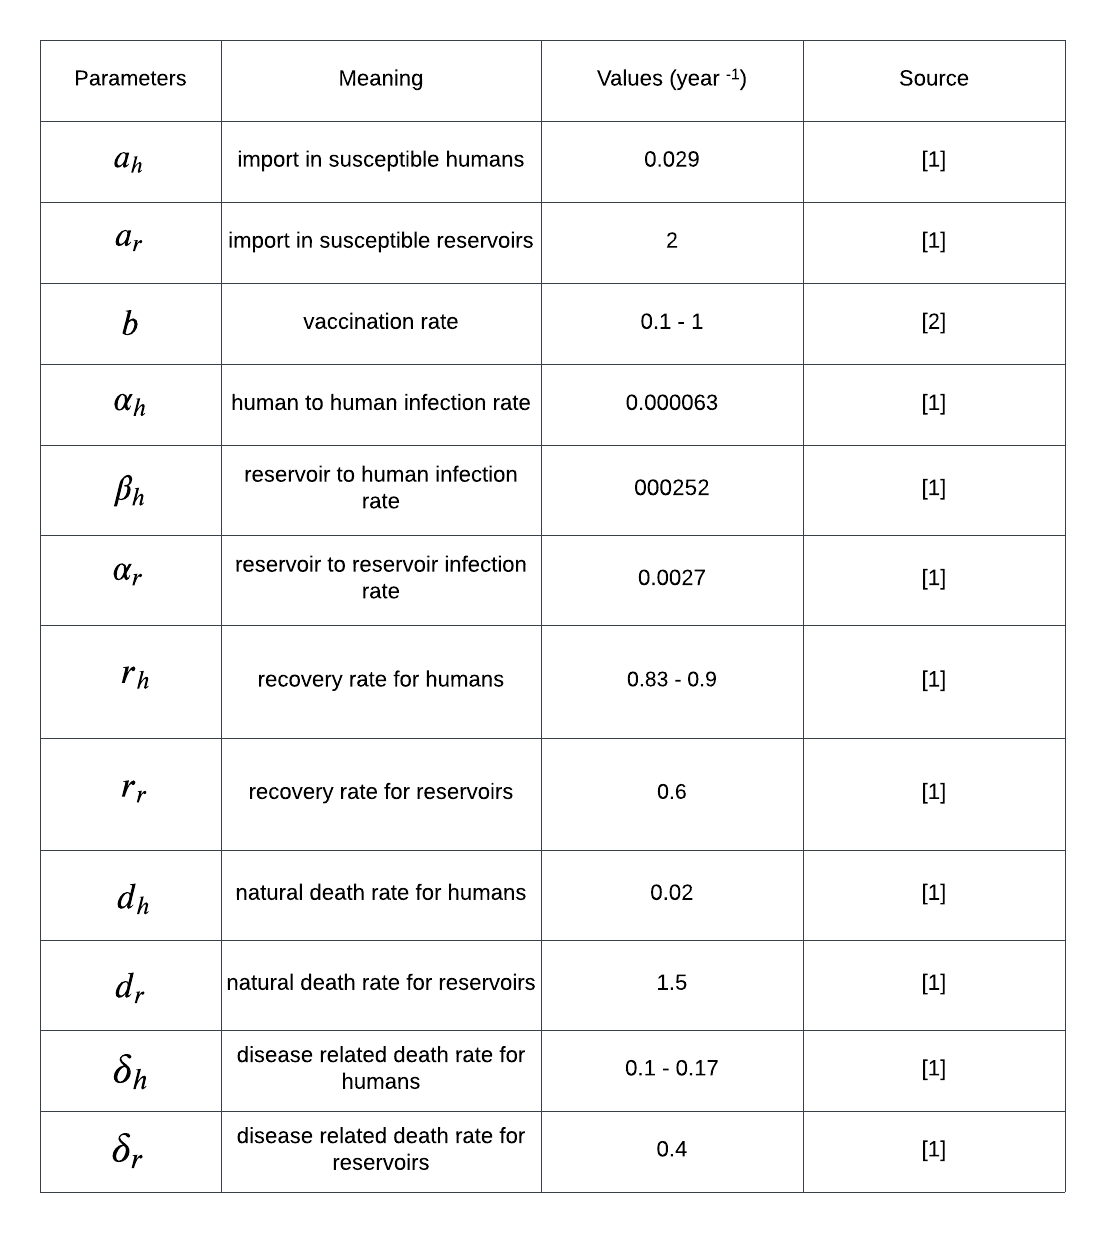
\includegraphics[scale=0.3]{parameters-table}
\caption{Parameters Table}
%\centering
\end{figure}

To allow for a general latent period, we further assume that $P(t)$ is the probability of individuals remaining in the vaccinated class $t$ units after being vaccinated and $Q(t)$ is the probability of individuals remaining in the exposed class $t$ units after being exposed to the monkeypox virus.
According to the natural progression of the disease, we assume $P(t)$ and $Q(t)$ non-negative, non-increasing and piecewise continuous with 
\begin{center}
$P(0^{+}) = Q(0^{+}) = 1$ and $P(\infty) = Q(\infty) = 0$
\end{center}

The number of individuals who become exposed at some time $\mu \in (0,t)$ and are still in the exposed class at time $t$ is given by
\begin{equation}
E_{h}(t) = \int_{0}^{t} (\alpha_{h}S_{h}(\mu)I_{h}(\mu) +\beta_{h}S_{h}(\mu)I_{r}(\mu)) e^{-d_{h}(t-\mu)}Q(t-\mu) \,d\mu \label{exposed}
\end{equation}


and the number of individuals who get vaccinated at some time $\mu \in (0,t)$ and are still in the vaccinated class at time $t$ is given by
\begin{equation}
V_{h}(t) = \int_{0}^{t} bS_{h}(\mu)e^{-d_{h}(t-\mu)}P(t-\mu) \,d\mu \label{vaccinated}
\end{equation}


%Now, substituting $v = t-\mu$, we get

%\[E_{h}(t) = \int_{0}^{t} (\beta_{h}S_{h}(t-v)I_{h}(t-v) + \alpha_{h}S_{h}(t-v)I_{r}(t-v)) e^{-d_{h}v}Q(v) \,dv\]

%\[V_{h}(t) = \int_{0}^{t} bS_{h}(t-v)e^{-d_{h}(v)}P(v) \,dv\]
The general model is represented as follows
\begin{align}
\begin{split}
S_{h}'(t) &= a_{h}-d_{h}S_{h}(t)-bS_{h}(t)-(\alpha_{h}S_{h}(t)I_{h}(t)+\beta_{h}S_{h}(t)I_{r}(t))\\
&-\int_{0}^{t} bS_{h}(\mu)e^{-d_{h}(t-\mu)}P'(t-\mu) \,d\mu
\end{split} \label{meq1}\\
%-------------------------------------------------------------
V_{h}'(t) &= bS_{h}(t)-d_{h}V_{h}(t)+\int_{0}^{t} bS_{h}(\mu)e^{-d_{h}(t-\mu)}P'(t-\mu) \,d\mu  \label{meq2}\\
%-------------------------------------------------------------
\begin{split}
E_{h}'(t) &= \alpha_{h}S_{h}(t)I_{h}(t)+\beta_{h}S_{h}(t)I_{r}(t))-d_{h}E_{h}(t)\\
&+\int_{0}^{t} (\alpha_{h}S_{h}(\mu)I_{h}(\mu)+\beta_{h}S_{h}(\mu)I_{r}(\mu))e^{-d_{h}(t-\mu)}Q'(t-\mu) \,d\mu  \end{split} \label{meq3}\\
%-------------------------------------------------------------
\begin{split}
I_{h}'(t) &= -\int_{0}^{t} (\alpha_{h}S_{h}(\mu)I_{h}(\mu)+\beta_{h}S_{h}(\mu)I_{r}(\mu))e^{-d_{h}(t-\mu)}Q'(t-\mu) \,d\mu -d_{h}I_{h}(t)\\
&-\delta_{h}I_{h}(t) -r_{h}I_{h}(t)
\end{split} \label{meq4}\\
%-------------------------------------------------------------
R_{h}'(t) &= r_{h}I_{h}(t) -d_{h}R_{h}(t) \label{meq5}\\ 
%-------------------------------------------------------------
S_{r}'(t) &= a_{r}-d_{r}S_{r}(t)-\alpha_{r}S_{r}(t)I_{r}(t)  \label{meq6}\\
%-------------------------------------------------------------
I_{r}'(t) &= \alpha_{r}S_{r}(t)I_{r}(t) -d_{r}I_{r}(t) -\delta_{r}I_{r}(t)- r_{r}I_{r}(t)  \label{meq7}\\
%-------------------------------------------------------------
R_{r}'(t) &= r_{r}I_{r}(t) -d_{r}R_{r}(t)  \label{meq8}
%-------------------------------------------------------------
\end{align}

To obtain more specific models, we have discussed four cases with different values for the functions $P(t)$ and $Q(t)$.

% CASE 1
Case \rom{1} [$P(t)=e^{-\omega_{1} t}, Q(t)=e^{-\omega_{2} t}$]

Equation \ref{exposed} becomes
\[E_{h}(t) = \int_{0}^{t} (\alpha_{h}S_{h}(\mu)I_{h}(\mu) + \beta_{h}S_{h}(\mu)I_{r}(\mu)) e^{(d_{h}+\omega_{2})\mu-(d_{h}+\omega_{2})t} \,d\mu\]
%-------------------------------------------------------------
\[\Rightarrow E_{h}(t) = e^{-(d_{h}+\omega_{2})t}\int_{0}^{t} (\alpha_{h}S_{h}(\mu)I_{h}(\mu) + \beta_{h}S_{h}(\mu)I_{r}(\mu)) e^{(d_{h}+\omega_{2})\mu} \,d\mu\]
%-------------------------------------------------------------
\[\Rightarrow E_{h}'(t) = -(d_{h}+\omega_{2})E_{h}(t) + e^{-(d_{h}+\omega_{2})t}(\alpha_{h}S_{h}(t)I_{h}(t) + \beta_{h}S_{h}(t)I_{r}(t)) e^{(d_{h}+\omega_{2})t}\]
%-------------------------------------------------------------
\[\Rightarrow E_{h}'(t) = \alpha_{h}S_{h}(t)I_{h}(t) + \beta_{h}S_{h}(t)I_{r}(t)-(d_{h}+\omega_{2})E_{h}(t)\]
%-------------------------------------------------------------
Again, equation \ref{vaccinated} becomes
\[V_{h}(t) = \int_{0}^{t} bS_{h}(\mu)e^{(d_{h}+\omega_{1})\mu-(d_{h}+\omega_{1})t} \,d\mu\]
%-------------------------------------------------------------
\[\Rightarrow V_{h}(t) = e^{-(d_{h}+\omega_{1})t}\int_{0}^{t} bS_{h}(\mu) e^{(d_{h}+\omega_{1})\mu} \,d\mu\]
%-------------------------------------------------------------
\[\Rightarrow V_{h}'(t) = -(d_{h}+\omega_{1})V_{h}(t) + e^{-(d_{h}+\omega_{1})t}bS_{h}(t) e^{(d_{h}+\omega_{1})t}\]
%-------------------------------------------------------------
\[\Rightarrow V_{h}'(t) = bS_{h}(t)-(d_{h}+\omega_{1})V_{h}(t)\]
%-------------------------------------------------------------
The model for case \rom{1} is represented as follows
\begin{flalign} 
S_{h}'(t) &= a_{h}+\omega_{1} V_{h}(t)-d_{h}S_{h}(t)-bS_{h}(t)-(\alpha_{h}S_{h}(t)I_{h}(t)+\beta_{h}S_{h}(t)I_{r}(t)) \label{case1meq1}\\
%-------------------------------------------------------------
V_{h}'(t) &= bS_{h}(t)-(d_{h}+\omega_{1})V_{h}(t) \label{case1meq2}\\
%-------------------------------------------------------------
E_{h}'(t) &= \alpha_{h}S_{h}(t)I_{h}(t) + \beta_{h}S_{h}(t)I_{r}(t)-(d_{h}+\omega_{2})E_{h}(t)  \label{case1meq3}\\
%-------------------------------------------------------------
I_{h}'(t) &= \omega_{2} E_{h}(t) -d_{h}I_{h}(t) -\delta_{h}I_{h}(t) -r_{h}I_{h}(t)  \label{case1meq4}\\
%-------------------------------------------------------------
R_{h}'(t) &= r_{h}I_{h}(t) -d_{h}R_{h}(t) \label{case1meq5}\\ 
%-------------------------------------------------------------
S_{r}'(t) &= a_{r}-d_{r}S_{r}(t)-\alpha_{r}S_{r}(t)I_{r}(t)  \label{case1meq6}\\
%-------------------------------------------------------------
I_{r}'(t) &= \alpha_{r}S_{r}(t)I_{r}(t) -d_{r}I_{r}(t) -\delta_{r}I_{r}(t)- r_{r}I_{r}(t)  \label{case1meq7}\\
%-------------------------------------------------------------
R_{r}'(t) &= r_{r}I_{r}(t) -d_{r}R_{r}(t)  \label{case1meq8}
%-------------------------------------------------------------
\end{flalign}

% CASE 2
Case \rom{2} $\Biggl[P(t)=e^{-\omega t}, Q(t)=\begin{cases}
        1 & \text{if } t \in (0,\tau]\\
        0 & \text{if } t > \tau
    \end{cases}\Biggr\}\Biggr]$\\
% when t lies in 0 and tau
when $t \in (0,\tau]$, equation \ref{exposed} becomes
\begin{flalign*}
E_{h}(t) &= \int_{0}^{t} (\alpha_{h}S_{h}(\mu)I_{h}(\mu) +\beta_{h}S_{h}(\mu)I_{r}(\mu)) e^{-d_{h}(t-\mu)} \,d\mu\\
%-------------------------------------------------------------
&= e^{-d_{h}t} \int_{0}^{t} (\alpha_{h}S_{h}(\mu)I_{h}(\mu) +\beta_{h}S_{h}(\mu)I_{r}(\mu)) e^{d_{h}\mu} \,d\mu\\
%-------------------------------------------------------------
\Rightarrow E_{h}'(t) &= -d_{h}E_{h}+\alpha_{h}S_{h}(t)I_{h}(t) +\beta_{h}S_{h}(t)I_{r}(t)
\end{flalign*}
Again, when $t \in (0,\tau]$, equation \ref{vaccinated} becomes
\begin{flalign*}
V_{h}(t) &= \int_{0}^{t} bS_{h}(\mu)e^{-d_{h}(t-\mu)}e^{-\omega(t-\mu)} \,d\mu\\
%-------------------------------------------------------------
&= e^{-(\omega+d_{h})t}\int_{0}^{t} bS_{h}(\mu)e^{(\omega+d_{h})\mu} \,d\mu\\
%-------------------------------------------------------------
\Rightarrow V_{h}'(t) &= bS_{h}t - (\omega+d_{h})V_{h}
\end{flalign*}
%-------------------------------------------------------------
The model for case \rom{2} when $t \in (0,\tau]$ is represented as follows
\begin{flalign} 
S_{h}'(t) &= a_{h}+\omega V_{h}(t)-d_{h}S_{h}(t)-bS_{h}(t)-(\alpha_{h}S_{h}(t)I_{h}(t)+\beta_{h}S_{h}(t)I_{r}(t)) \label{case1meq1}\\
%-------------------------------------------------------------
V_{h}'(t) &= bS_{h}t - (\omega+d_{h})V_{h} \label{case1meq2}\\
%-------------------------------------------------------------
E_{h}'(t) &= -d_{h}E_{h}+\alpha_{h}S_{h}(t)I_{h}(t) +\beta_{h}S_{h}(t)I_{r}(t)  \label{case1meq3}\\
%-------------------------------------------------------------
I_{h}'(t) &= -(d_{h}+\delta_{h}+r_{h})I_{h}(t)  \label{case1meq4}\\
%-------------------------------------------------------------
R_{h}'(t) &= r_{h}I_{h}(t) -d_{h}R_{h}(t) \label{case1meq5}\\ 
%-------------------------------------------------------------
S_{r}'(t) &= a_{r}-d_{r}S_{r}(t)-\alpha_{r}S_{r}(t)I_{r}(t)  \label{case1meq6}\\
%-------------------------------------------------------------
I_{r}'(t) &= \alpha_{r}S_{r}(t)I_{r}(t) -(d_{r}+\delta_{r}+r_{r})I_{r}(t) \label{case1meq7}\\
%-------------------------------------------------------------
R_{r}'(t) &= r_{r}I_{r}(t) -d_{r}R_{r}(t)  \label{case1meq8}
%-------------------------------------------------------------
\end{flalign}
% when t > tau
when $t > \tau$, equation \ref{exposed} becomes
\begin{flalign*}
E_{h}(t) &= \int_{t-\tau}^{t} (\alpha_{h}S_{h}(\mu)I_{h}(\mu) +\beta_{h}S_{h}(\mu)I_{r}(\mu)) e^{-d_{h}(t-\mu)} \,d\mu\\
%-------------------------------------------------------------
&= e^{-d_{h}t} \int_{t-\tau}^{t} (\alpha_{h}S_{h}(\mu)I_{h}(\mu) +\beta_{h}S_{h}(\mu)I_{r}(\mu)) e^{d_{h}\mu} \,d\mu\\
%-------------------------------------------------------------
\Rightarrow E_{h}'(t) &= -d_{h}E_{h}+\alpha_{h}S_{h}(t)I_{h}(t) +\beta_{h}S_{h}(t)I_{r}(t)-\biggl[\alpha_{h}S_{h}(t-\tau)I_{h}(t-\tau) +\beta_{h}S_{h}(t-\tau)I_{r}(t-\tau)\biggr]e^{-d_{h}\tau}
\end{flalign*}
Again, when $t > \tau$, equation \ref{vaccinated} becomes
\begin{flalign*}
V_{h}(t) &= \int_{0}^{t} bS_{h}(\mu)e^{-d_{h}(t-\mu)}e^{-\omega(t-\mu)} \,d\mu\\
%-------------------------------------------------------------
&= e^{-(\omega+d_{h})t}\int_{0}^{t} bS_{h}(\mu)e^{(\omega+d_{h})\mu} \,d\mu\\
%-------------------------------------------------------------
\Rightarrow V_{h}'(t) &= bS_{h}t - (\omega+d_{h})V_{h}
\end{flalign*}
%-------------------------------------------------------------
The model for case \rom{2} when $t > \tau$ is represented as follows
\begin{flalign} 
S_{h}'(t) &= a_{h}+\omega V_{h}(t)-d_{h}S_{h}(t)-bS_{h}(t)-(\alpha_{h}S_{h}(t)I_{h}(t)+\beta_{h}S_{h}(t)I_{r}(t)) \\
%-------------------------------------------------------------
V_{h}'(t) &= bS_{h}t - (\omega+d_{h})V_{h} \\
%-------------------------------------------------------------
E_{h}'(t) &= -d_{h}E_{h}+\alpha_{h}S_{h}(t)I_{h}(t) +\beta_{h}S_{h}(t)I_{r}(t)-\biggl[\alpha_{h}S_{h}(t-\tau)I_{h}(t-\tau) +\beta_{h}S_{h}(t-\tau)I_{r}(t-\tau)\biggr]e^{-d_{h}\tau}\\
%-------------------------------------------------------------
I_{h}'(t) &= \biggl[\alpha_{h}S_{h}(t-\tau)I_{h}(t-\tau) +\beta_{h}S_{h}(t-\tau)I_{r}(t-\tau)\biggr]e^{-d_{h}\tau} -(d_{h}+\delta_{h}+r_{h})I_{h}(t)\\
%-------------------------------------------------------------
R_{h}'(t) &= r_{h}I_{h}(t) -d_{h}R_{h}(t)\\ 
%-------------------------------------------------------------
S_{r}'(t) &= a_{r}-d_{r}S_{r}(t)-\alpha_{r}S_{r}(t)I_{r}(t)\\
%-------------------------------------------------------------
I_{r}'(t) &= \alpha_{r}S_{r}(t)I_{r}(t) -(d_{r}+\delta_{r}+r_{r})I_{r}(t)\\
%-------------------------------------------------------------
R_{r}'(t) &= r_{r}I_{r}(t) -d_{r}R_{r}(t)
%-------------------------------------------------------------
\end{flalign}

% CASE 3
Case \rom{3} $\Biggl[P(t)=\begin{cases}
        1 & \text{if } t \in (0,\tau]\\
        0 & \text{if } t > \tau
    \end{cases}\Biggr\}, Q(t)=e^{-\omega t}\Biggr]$\\
% when t lies in 0 and tau
when $t \in (0,\tau]$, equation \ref{exposed} becomes
\begin{flalign*}
E_{h}(t) &= \int_{0}^{t} (\alpha_{h}S_{h}(\mu)I_{h}(\mu) +\beta_{h}S_{h}(\mu)I_{r}(\mu)) e^{-d_{h}(t-\mu)}e^{-\omega(t-\mu)} \,d\mu\\
%-------------------------------------------------------------
&= e^{-(\omega+d_{h})t} \int_{0}^{t} (\alpha_{h}S_{h}(\mu)I_{h}(\mu) +\beta_{h}S_{h}(\mu)I_{r}(\mu)) e^{(\omega+d_{h})\mu} \,d\mu\\
%-------------------------------------------------------------
\Rightarrow E_{h}'(t) &= -(\omega+d_{h})E_{h}+\alpha_{h}S_{h}(t)I_{h}(t) +\beta_{h}S_{h}(t)I_{r}(t)
\end{flalign*}
Again, when $t \in (0,\tau]$, equation \ref{vaccinated} becomes
\begin{flalign*}
V_{h}(t) &= \int_{0}^{t} bS_{h}(\mu)e^{-d_{h}(t-\mu)} \,d\mu\\
%-------------------------------------------------------------
&= e^{-d_{h}t}\int_{0}^{t} bS_{h}(\mu)e^{d_{h}\mu} \,d\mu\\
%-------------------------------------------------------------
\Rightarrow V_{h}'(t) &= bS_{h}(t) - d_{h}V_{h}
\end{flalign*}
%-------------------------------------------------------------
The model for case \rom{3} when $t \in (0,\tau]$ is represented as follows
\begin{flalign} 
S_{h}'(t) &= a_{h}-d_{h}S_{h}(t)-bS_{h}(t)-(\alpha_{h}S_{h}(t)I_{h}(t)+\beta_{h}S_{h}(t)I_{r}(t))\\
%-------------------------------------------------------------
V_{h}'(t) &= bS_{h}t - d_{h}V_{h}\\
%-------------------------------------------------------------
E_{h}'(t) &= -(\omega+d_{h})E_{h}+\alpha_{h}S_{h}(t)I_{h}(t) +\beta_{h}S_{h}(t)I_{r}(t)\\
%-------------------------------------------------------------
I_{h}'(t) &= \omega E_{h}-(d_{h}+\delta_{h}+r_{h})I_{h}(t)\\
%-------------------------------------------------------------
R_{h}'(t) &= r_{h}I_{h}(t) -d_{h}R_{h}(t)\\ 
%-------------------------------------------------------------
S_{r}'(t) &= a_{r}-d_{r}S_{r}(t)-\alpha_{r}S_{r}(t)I_{r}(t)\\
%-------------------------------------------------------------
I_{r}'(t) &= \alpha_{r}S_{r}(t)I_{r}(t) -(d_{r}+\delta_{r}+r_{r})I_{r}(t)\\
%-------------------------------------------------------------
R_{r}'(t) &= r_{r}I_{r}(t) -d_{r}R_{r}(t)
%-------------------------------------------------------------
\end{flalign}
% when t > tau
when $t > \tau$, equation \ref{exposed} becomes
\begin{flalign*}
E_{h}(t) &= \int_{0}^{t} (\alpha_{h}S_{h}(\mu)I_{h}(\mu) +\beta_{h}S_{h}(\mu)I_{r}(\mu)) e^{-d_{h}(t-\mu)}e^{-\omega(t-\mu)} \,d\mu\\
%-------------------------------------------------------------
&= e^{-(\omega+d_{h})t} \int_{0}^{t} (\alpha_{h}S_{h}(\mu)I_{h}(\mu) +\beta_{h}S_{h}(\mu)I_{r}(\mu)) e^{(\omega+d_{h})\mu} \,d\mu\\
%-------------------------------------------------------------
\Rightarrow E_{h}'(t) &= -(d_{h}+\omega)E_{h}+\alpha_{h}S_{h}(t)I_{h}(t) +\beta_{h}S_{h}(t)I_{r}(t)
\end{flalign*}
Again, when $t > \tau$, equation \ref{vaccinated} becomes
\begin{flalign*}
V_{h}(t) &= \int_{t-\tau}^{t} bS_{h}(\mu)e^{-d_{h}(t-\mu)} \,d\mu\\
%-------------------------------------------------------------
&= e^{-d_{h}t}\int_{t-\tau}^{t} bS_{h}(\mu)e^{d_{h}\mu} \,d\mu\\
%-------------------------------------------------------------
\Rightarrow V_{h}'(t) &= bS_{h}(t) - d_{h}V_{h} - bS_{h}(t-\tau)e^{-d_{h}\tau}
\end{flalign*}
%-------------------------------------------------------------
The model for case \rom{3} when $t > \tau$ is represented as follows
\begin{flalign} 
S_{h}'(t) &= a_{h}-d_{h}S_{h}(t)-bS_{h}(t) + bS_{h}(t-\tau)e^{-d_{h}\tau} -(\alpha_{h}S_{h}(t)I_{h}(t)+\beta_{h}S_{h}(t)I_{r}(t)) \\
%-------------------------------------------------------------
V_{h}'(t) &= bS_{h}(t) - d_{h}V_{h} - bS_{h}(t-\tau)e^{-d_{h}\tau} \\
%-------------------------------------------------------------
E_{h}'(t) &= -(d_{h}+\omega)E_{h}+\alpha_{h}S_{h}(t)I_{h}(t) +\beta_{h}S_{h}(t)I_{r}(t)\\
%-------------------------------------------------------------
I_{h}'(t) &= \omega  E_{h} -(d_{h}+\delta_{h}+r_{h})I_{h}(t)\\
%-------------------------------------------------------------
R_{h}'(t) &= r_{h}I_{h}(t) -d_{h}R_{h}(t)\\ 
%-------------------------------------------------------------
S_{r}'(t) &= a_{r}-d_{r}S_{r}(t)-\alpha_{r}S_{r}(t)I_{r}(t)\\
%-------------------------------------------------------------
I_{r}'(t) &= \alpha_{r}S_{r}(t)I_{r}(t) -(d_{r}+\delta_{r}+r_{r})I_{r}(t)\\
%-------------------------------------------------------------
R_{r}'(t) &= r_{r}I_{r}(t) -d_{r}R_{r}(t)
%-------------------------------------------------------------
\end{flalign}

% CASE 4
Case \rom{4} $\Biggl[P(t)=\begin{cases}
        1 & \text{if } t \in (0,\tau_{1}]\\
        0 & \text{if } t > \tau_{1}
    \end{cases}\Biggr\}, Q(t)=\begin{cases}
        1 & \text{if } t \in (0,\tau_{2}]\\
        0 & \text{if } t > \tau_{2}
    \end{cases}\Biggr\}\Biggr]$\\
without the loss of generality, we assume that $\tau_{1}<\tau_{2}$.\\
% when t < min{tau1, tau2}
when $t < \min\{\tau_{1}, \tau_{2}\}$, equation \ref{exposed} becomes
\begin{flalign*}
E_{h}(t) &= \int_{0}^{t} (\alpha_{h}S_{h}(\mu)I_{h}(\mu) +\beta_{h}S_{h}(\mu)I_{r}(\mu)) e^{-d_{h}(t-\mu)} \,d\mu\\
%-------------------------------------------------------------
\Rightarrow E_{h}'(t) &= -d_{h}E_{h}+\alpha_{h}S_{h}(t)I_{h}(t) +\beta_{h}S_{h}(t)I_{r}(t)
\end{flalign*}
Again, when $t < \min\{\tau_{1}, \tau_{2}\}$, equation \ref{vaccinated} becomes
\begin{flalign*}
V_{h}(t) &= \int_{0}^{t} bS_{h}(\mu)e^{-d_{h}(t-\mu)} \,d\mu\\
%-------------------------------------------------------------
&= e^{-d_{h}t}\int_{0}^{t} bS_{h}(\mu)e^{d_{h}\mu} \,d\mu\\
%-------------------------------------------------------------
\Rightarrow V_{h}'(t) &= bS_{h}(t) - d_{h}V_{h}
\end{flalign*}
%-------------------------------------------------------------
The model for case \rom{4} when $t < \min\{\tau_{1}, \tau_{2}\}$ is represented as follows
\begin{flalign} 
S_{h}'(t) &= a_{h}-d_{h}S_{h}(t)-bS_{h}(t)-(\alpha_{h}S_{h}(t)I_{h}(t)+\beta_{h}S_{h}(t)I_{r}(t))\\
%-------------------------------------------------------------
V_{h}'(t) &= bS_{h}t - d_{h}V_{h}\\
%-------------------------------------------------------------
E_{h}'(t) &= -d_{h}E_{h}+\alpha_{h}S_{h}(t)I_{h}(t) +\beta_{h}S_{h}(t)I_{r}(t)\\
%-------------------------------------------------------------
I_{h}'(t) &= -(d_{h}+\delta_{h}+r_{h})I_{h}(t)\\
%-------------------------------------------------------------
R_{h}'(t) &= r_{h}I_{h}(t) -d_{h}R_{h}(t)\\ 
%-------------------------------------------------------------
S_{r}'(t) &= a_{r}-d_{r}S_{r}(t)-\alpha_{r}S_{r}(t)I_{r}(t)\\
%-------------------------------------------------------------
I_{r}'(t) &= \alpha_{r}S_{r}(t)I_{r}(t) -(d_{r}+\delta_{r}+r_{r})I_{r}(t)\\
%-------------------------------------------------------------
R_{r}'(t) &= r_{r}I_{r}(t) -d_{r}R_{r}(t)
%-------------------------------------------------------------
\end{flalign}
% when min{tau1, tau2} < t < max{tau1, tau2}
when $\min\{\tau_{1}, \tau_{2}\} < t < \max\{\tau_{1}, \tau_{2}\}$, equation \ref{exposed} becomes
\begin{flalign*}
E_{h}(t) &= \int_{0}^{t} (\alpha_{h}S_{h}(\mu)I_{h}(\mu) +\beta_{h}S_{h}(\mu)I_{r}(\mu)) e^{-d_{h}(t-\mu)} \,d\mu\\
%-------------------------------------------------------------
&= e^{-d_{h}t} \int_{0}^{t} (\alpha_{h}S_{h}(\mu)I_{h}(\mu) +\beta_{h}S_{h}(\mu)I_{r}(\mu)) e^{d_{h}\mu} \,d\mu\\
%-------------------------------------------------------------
\Rightarrow E_{h}'(t) &= -d_{h}E_{h}+\alpha_{h}S_{h}(t)I_{h}(t) +\beta_{h}S_{h}(t)I_{r}(t)
\end{flalign*}
Again, when $\min\{\tau_{1}, \tau_{2}\} < t < \max\{\tau_{1}, \tau_{2}\}$, equation \ref{vaccinated} becomes
\begin{flalign*}
V_{h}(t) &= \int_{t-\tau_{1}}^{t} bS_{h}(\mu)e^{-d_{h}(t-\mu)} \,d\mu\\
%-------------------------------------------------------------
&= e^{-d_{h}t}\int_{t-\tau_{1}}^{t} bS_{h}(\mu)e^{d_{h}\mu} \,d\mu\\
%-------------------------------------------------------------
\Rightarrow V_{h}'(t) &= bS_{h}(t) - d_{h}V_{h} - bS_{h}(t-\tau_{1})e^{-d_{h}\tau_{1}}
\end{flalign*}
%-------------------------------------------------------------
The model for case \rom{4} when $\min\{\tau_{1}, \tau_{2}\} < t < \max\{\tau_{1}, \tau_{2}\}$ is represented as follows
\begin{flalign}
S_{h}'(t) &= a_{h}-d_{h}S_{h}(t)-bS_{h}(t) + bS_{h}(t-\tau_{1})e^{-d_{h}\tau_{1}} -(\alpha_{h}S_{h}(t)I_{h}(t)+\beta_{h}S_{h}(t)I_{r}(t)) \\
%-------------------------------------------------------------
V_{h}'(t) &= bS_{h}(t) - d_{h}V_{h} - bS_{h}(t-\tau_{1})e^{-d_{h}\tau_{1}} \\
%-------------------------------------------------------------
E_{h}'(t) &= -d_{h}E_{h}+\alpha_{h}S_{h}(t)I_{h}(t) +\beta_{h}S_{h}(t)I_{r}(t)\\
%-------------------------------------------------------------
I_{h}'(t) &= -(d_{h}+\delta_{h}+r_{h})I_{h}(t)\\
%-------------------------------------------------------------
R_{h}'(t) &= r_{h}I_{h}(t) -d_{h}R_{h}(t)\\ 
%-------------------------------------------------------------
S_{r}'(t) &= a_{r}-d_{r}S_{r}(t)-\alpha_{r}S_{r}(t)I_{r}(t)\\
%-------------------------------------------------------------
I_{r}'(t) &= \alpha_{r}S_{r}(t)I_{r}(t) -(d_{r}+\delta_{r}+r_{r})I_{r}(t)\\
%-------------------------------------------------------------
R_{r}'(t) &= r_{r}I_{r}(t) -d_{r}R_{r}(t)
%-------------------------------------------------------------
\end{flalign}
% when t > max{tau1, tau2}
when $t > \max\{\tau_{1}, \tau_{2}\}$, equation \ref{exposed} becomes
\begin{flalign*}
E_{h}(t) &= \int_{t-\tau_{2}}^{t} (\alpha_{h}S_{h}(\mu)I_{h}(\mu) +\beta_{h}S_{h}(\mu)I_{r}(\mu)) e^{-d_{h}(t-\mu)} \,d\mu\\
%-------------------------------------------------------------
&= e^{-d_{h}t} \int_{t-\tau_{2}}^{t} (\alpha_{h}S_{h}(\mu)I_{h}(\mu) +\beta_{h}S_{h}(\mu)I_{r}(\mu)) e^{d_{h}\mu} \,d\mu\\
%-------------------------------------------------------------
\Rightarrow E_{h}'(t) &= -d_{h}E_{h}+\alpha_{h}S_{h}(t)I_{h}(t) +\beta_{h}S_{h}(t)I_{r}(t) - \Bigl[\alpha_{h}S_{h}(t-\tau_{2})I_{h}(t-\tau_{2}) +\beta_{h}S_{h}(t-\tau_{2})I_{r}(t-\tau_{2})\Bigr]e^{-d_{h}\tau_{2}}
\end{flalign*}
Again, when $t > \max\{\tau_{1}, \tau_{2}\}$, equation \ref{vaccinated} becomes
\begin{flalign*}
V_{h}(t) &= \int_{t-\tau_{1}}^{t} bS_{h}(\mu)e^{-d_{h}(t-\mu)} \,d\mu\\
%-------------------------------------------------------------
&= e^{-d_{h}t}\int_{t-\tau_{1}}^{t} bS_{h}(\mu)e^{d_{h}\mu} \,d\mu\\
%-------------------------------------------------------------
\Rightarrow V_{h}'(t) &= bS_{h}(t) - d_{h}V_{h} - bS_{h}(t-\tau_{1})e^{-d_{h}\tau_{1}}
\end{flalign*}
%-------------------------------------------------------------
The model for case \rom{4} when $t > \max\{\tau_{1}, \tau_{2}\}$ is represented as follows
\begin{flalign}
S_{h}'(t) &= a_{h}-d_{h}S_{h}(t)-bS_{h}(t) + bS_{h}(t-\tau_{1})e^{-d_{h}\tau_{1}} -(\alpha_{h}S_{h}(t)I_{h}(t)+\beta_{h}S_{h}(t)I_{r}(t)) \\
%-------------------------------------------------------------
V_{h}'(t) &= bS_{h}(t) - d_{h}V_{h} - bS_{h}(t-\tau_{1})e^{-d_{h}\tau_{1}} \\
%-------------------------------------------------------------
E_{h}'(t) &= -d_{h}E_{h}+\alpha_{h}S_{h}(t)I_{h}(t) +\beta_{h}S_{h}(t)I_{r}(t) - \Bigl[\alpha_{h}S_{h}(t-\tau_{2})I_{h}(t-\tau_{2}) +\beta_{h}S_{h}(t-\tau_{2})I_{r}(t-\tau_{2})\Bigr]e^{-d_{h}\tau_{2}}\\
%-------------------------------------------------------------
I_{h}'(t) &= \Bigl[\alpha_{h}S_{h}(t-\tau_{2})I_{h}(t-\tau_{2}) +\beta_{h}S_{h}(t-\tau_{2})I_{r}(t-\tau_{2})\Bigr]e^{-d_{h}\tau_{2}} -(d_{h}+\delta_{h}+r_{h})I_{h}(t)\\
%-------------------------------------------------------------
R_{h}'(t) &= r_{h}I_{h}(t) -d_{h}R_{h}(t)\\ 
%-------------------------------------------------------------
S_{r}'(t) &= a_{r}-d_{r}S_{r}(t)-\alpha_{r}S_{r}(t)I_{r}(t)\\
%-------------------------------------------------------------
I_{r}'(t) &= \alpha_{r}S_{r}(t)I_{r}(t) -(d_{r}+\delta_{r}+r_{r})I_{r}(t)\\
%-------------------------------------------------------------
R_{r}'(t) &= r_{r}I_{r}(t) -d_{r}R_{r}(t)
%-------------------------------------------------------------
\end{flalign}